This section describes the features of {20-sim 4C} \cite{20sim4C} \footnote{Note that 20-sim 4C is Windows-only, but it can be executed using Wine \cite{winehq2016} on other platforms.} developed specifically in support of INTO-CPS and FMI.
%
{20-sim 4C} is a rapid prototyping tool that facilitates running C code on hardware to control machines and systems.
%
{20-sim 4C} imports models (as generated C code) from multiple sources (\emph{e.\@g.\@} 20-sim) and runs them on hardware targets such as embedded ARM boards (\emph{e.\@g.\@} Raspberry Pi), PCs running real-time Linux and industrial PLCs.

One of the goals of the \into project is to extend the capabilities of the \into tool chain toward executing part of a co-simulation on real hardware in real-time.
%
This is known as Hardware-in-the-Loop (HiL) simulation.
%
This section explains how the FMI import and export features of {20-sim 4C} can be used to execute source code FMUs on hardware targets in co-simulation under the control of the COE.
%
The complete {20-sim} tool documentation can be found in the {20-sim 4C} Reference Manual \cite{20sim4CManual13a}.
%
All details of the implementation of FMI support in 20-sim 4C can be found in Deliverable D4.3b \cite{INTOCPSD4.3b}.
%
%
%
\subsubsection{Source Code FMU Import}\label{sec:simulators:20sim4C:fmuimport}
To import an FMU in {20-sim 4C}, it must first be converted to a valid {20-sim 4C} project.
%
This is currently done via a command line call at the Windows Command prompt.
%
The command to import a source code FMU in {20-sim 4C} is:
%
%
%
\begin{quote}
\texttt{C:\textbackslash{}Program Files (x86)\textbackslash{}20-sim 4C 2.2\textbackslash{}bin\textbackslash{}\\20simparser.exe newfmuProjectName fmuFilename.fmu}\\
\end{quote}
%
%
%
where \texttt{newfmuProjectName} is the name of a new directory in which {20-sim 4C} will generate the new project.
%
This directory is created as a subdirectory of the current directory.
%
An example is shown in \autoref{figure:20-sim-4C_fmu_import1}.
%
%
%
\begin{figure}[hpt]
	\centerline{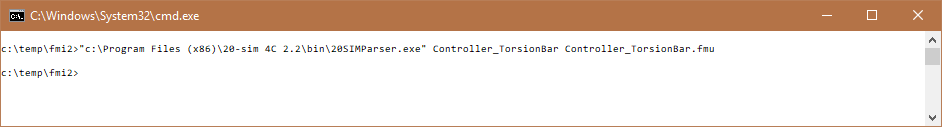
\includegraphics[width=\textwidth]{figures/20-sim-4C_fmu_import1.png}}
	\caption{Import a source code FMU in 20-sim 4C.}
	\label{figure:20-sim-4C_fmu_import1}
\end{figure}
%
%
%
This example creates a new directory in \texttt{C:\textbackslash{}Temp\textbackslash{}fmi2} named \texttt{Controller\_TorsionBar} and briefly shows the import dialog from \autoref{figure:20-sim-4C_fmu_import2}.
%
%
%
\begin{figure}[hpt]
	\centerline{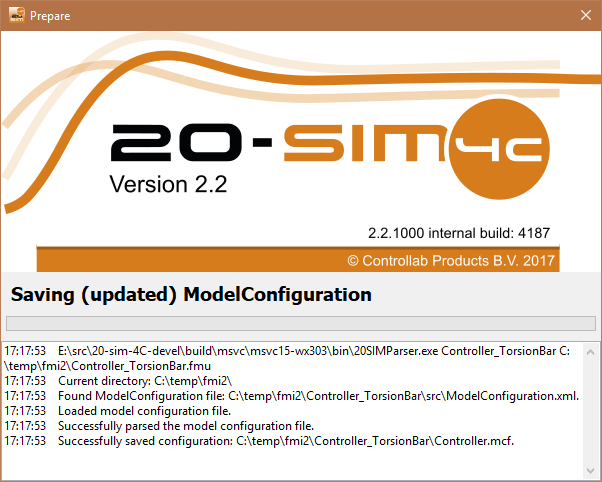
\includegraphics[width=0.8\textwidth]{figures/20-sim-4C_fmu_import2.png}}
	\caption{20-sim 4C FMU importer.}
	\label{figure:20-sim-4C_fmu_import2}
\end{figure}
%
%
%
After successfully extracting and importing the FMU, 20-sim 4C will start.

Source code FMUs are deployed to a real-time target as follows:
%
%
%
\begin{enumerate}
\item The 20-sim 4C window (\autoref{figure:20-sim-4C_select_target}) shows the name of the FMU and its public variables and parameters in the tree at the left side.
% 
\begin{figure}[hpt]
	\centerline{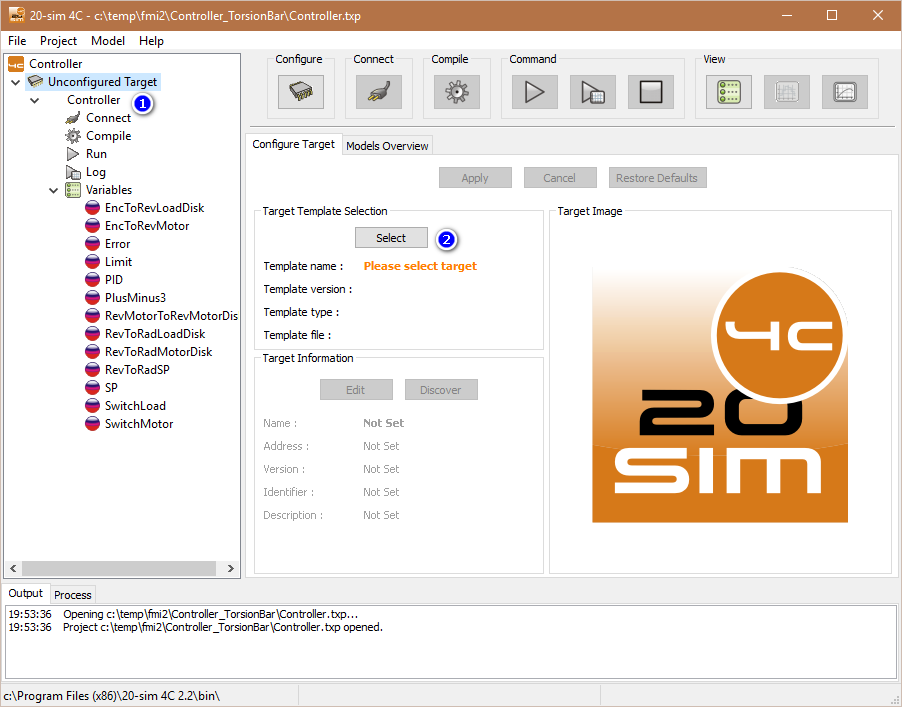
\includegraphics[width=\textwidth]{figures/20-sim-4C_select_target.png}}
	\caption{20-sim 4C project with imported FMU.}
	\label{figure:20-sim-4C_select_target}
\end{figure}
%
\item Use the \textit{Select} button in the \textit{Target Template Selection} box to select the hardware target for the FMU.  This shows the \textit{Select Target Configuration} dialog (\autoref{figure:20-sim-4C_select_raspberry_pi}.)
%
\begin{figure}[hpt]
	\centerline{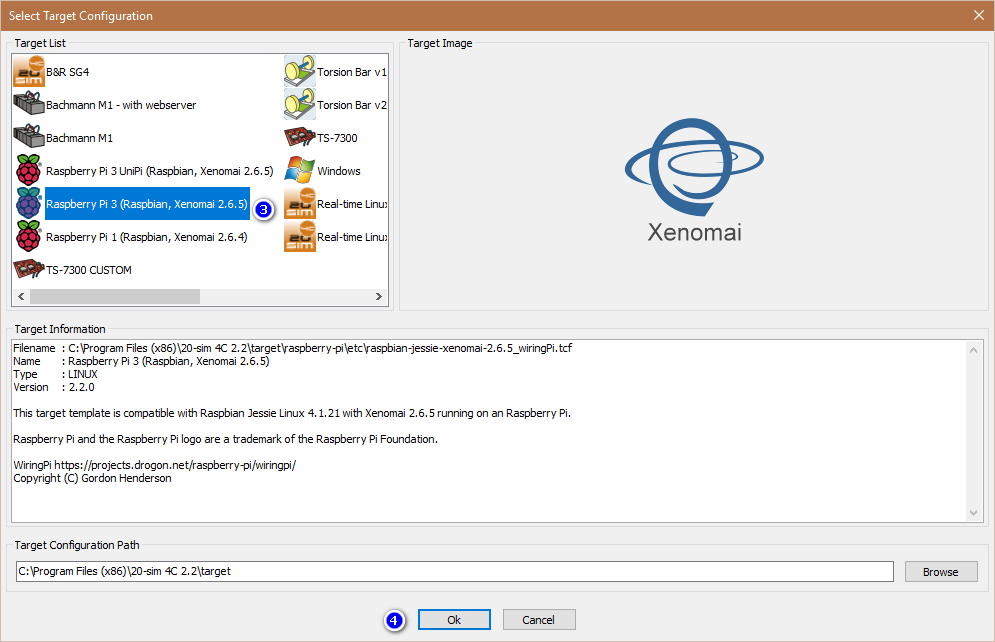
\includegraphics[width=\textwidth]{figures/20-sim-4C_select_raspberry_pi.png}}
	\caption{Select the Raspberry Pi target.}
	\label{figure:20-sim-4C_select_raspberry_pi}
\end{figure}
%
\item Select the \textit{Raspberry Pi 3 (Raspbian, Xenomai 2.6.5)} target.
\item Press the \textit{OK} button to confirm. This will automatically trigger a network scan to find the Raspberry Pi on the network.
\item In case multiple targets are found, select the desired target in the \textit{Please select a target} dialog (\autoref{figure:20-sim-4C_select_multiple_targets}) and press \textit{OK}.
%
%
%
\begin{figure}[hpt]
	\centerline{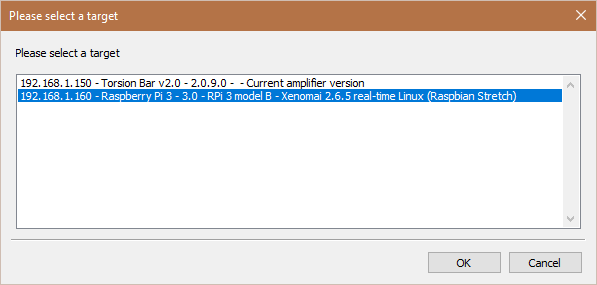
\includegraphics[width=0.8\textwidth]{figures/20-sim-4C_select_multiple_targets.png}}
	\caption{Select the right target.}
	\label{figure:20-sim-4C_select_multiple_targets}
\end{figure}
%
\item In the main 20-sim 4C window, press \textit{Apply} to confirm the target settings.  20-sim 4C will now try to connect to the Raspberry Pi. When the connection is successful, the \textit{Configure} button will turn green.
  See \autoref{figure:20-sim-4C_connect}.
%
\begin{figure}[hpt]
	\centerline{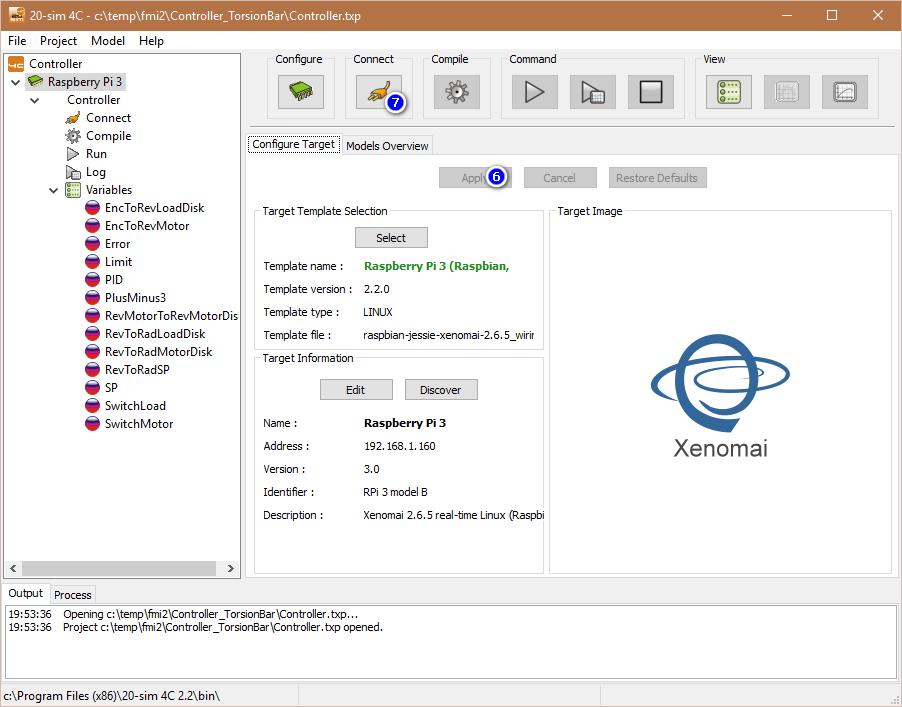
\includegraphics[width=\textwidth]{figures/20-sim-4C_connect.png}}
	\caption{Accept target settings and go to the connection phase.}
	\label{figure:20-sim-4C_connect}
\end{figure}
%
\item Click the \textit{Connect} button to go to the connection phase. This will show the inputs and outputs of the FMU and 20-sim 4C allows you to connect them to the on-board I/O pins.
%
\item To connect an input or output,  select the signal and press the \textit{Connect} button or double-click the signal (\autoref{figure:20-sim-4C_connect_io}.)  This will show the \textit{Connection} dialog as shown in \autoref{figure:20-sim-4C_connect_select_component}.
%
\begin{figure}[hpt]
	\centerline{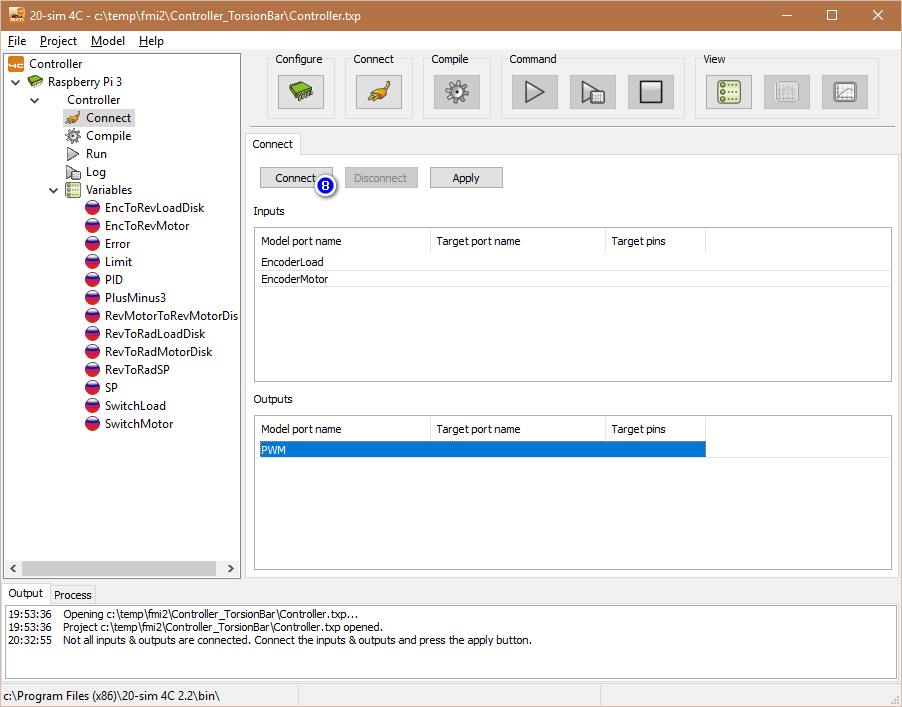
\includegraphics[width=\textwidth]{figures/20-sim-4C_connect_io.png}}
	\caption{Select an input or output and press \emph{Connect}.}
	\label{figure:20-sim-4C_connect_io}
\end{figure}
%
\item The connection dialog allows you to select an I/O component (\emph{e.\@g.\@} GPIO for digital I/O or PWM; see \autoref{figure:20-sim-4C_connect_select_component}) and a port within this component (typically a physical pin or connector on the target device; see \autoref{figure:20-sim-4C_connect_select_port}).  Select \textit{OK} to confirm the connection.  The I/O available depends on the selected target device.  The Raspberry Pi 3 provides by default only digital inputs and outputs and 2 PWM outputs.  Extension boards are needed for other I/O.\\
  \textbf{\textit{Note:}}  In case you would like to use an extension board or external I2C or SPI based I/O chip or other I/O, feel free to ask Controllab for options to support this in 20-sim 4C.
%
\begin{figure}[hpt]
	\centerline{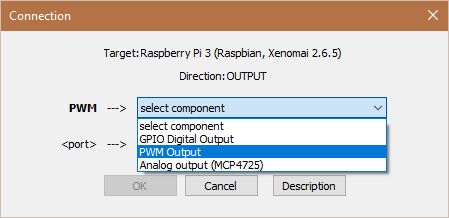
\includegraphics[width=0.6\textwidth]{figures/20-sim-4C_connect_select_component.png}}
	\caption{Select a component.}
	\label{figure:20-sim-4C_connect_select_component}
\end{figure}
%
\begin{figure}[hpt]
	\centerline{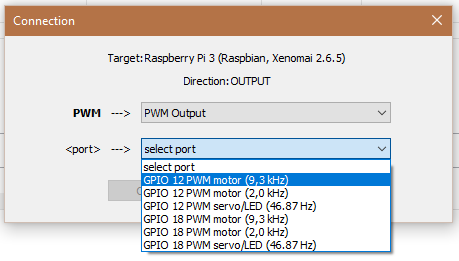
\includegraphics[width=0.6\textwidth]{figures/20-sim-4C_connect_select_port.png}}
	\caption{Select a port.}
	\label{figure:20-sim-4C_connect_select_port}
\end{figure}
%
\item When you have connected all desired inputs and outputs to the I/O, press the \textit{Apply} button (\autoref{figure:20-sim-4C_connect_apply}.)  The \textit{Connect} button will turn green and 20-sim 4C will extend the FMU source code with additional files to provide support for the Raspberry Pi Xenomai real-time Linux and the Raspberry Pi I/O.\\
%
\textbf{\textit{Note:}} It is not required to connect all inputs and outputs to real I/O.  20-sim 4C will show a warning when some inputs or outputs are not connected.  Unconnected inputs will read a zero (0) value by default.  A special real-time toolwrapper FMU can be generated from 20-sim 4C that will allow you to write to unconnected inputs from a co-simulation experiment (see section \ref{sec:simulators:20sim4C:fmuexport}).  This toolwrapper FMU will also allow you to read all FMU exported variables including all inputs and outputs even when inputs and outputs are connected to the I/O.  This toolwrapper FMU is the basis for INTO-CPS HiL simulation with the Raspberry Pi as the real-time target.
%
\begin{figure}[hpt]
	\centerline{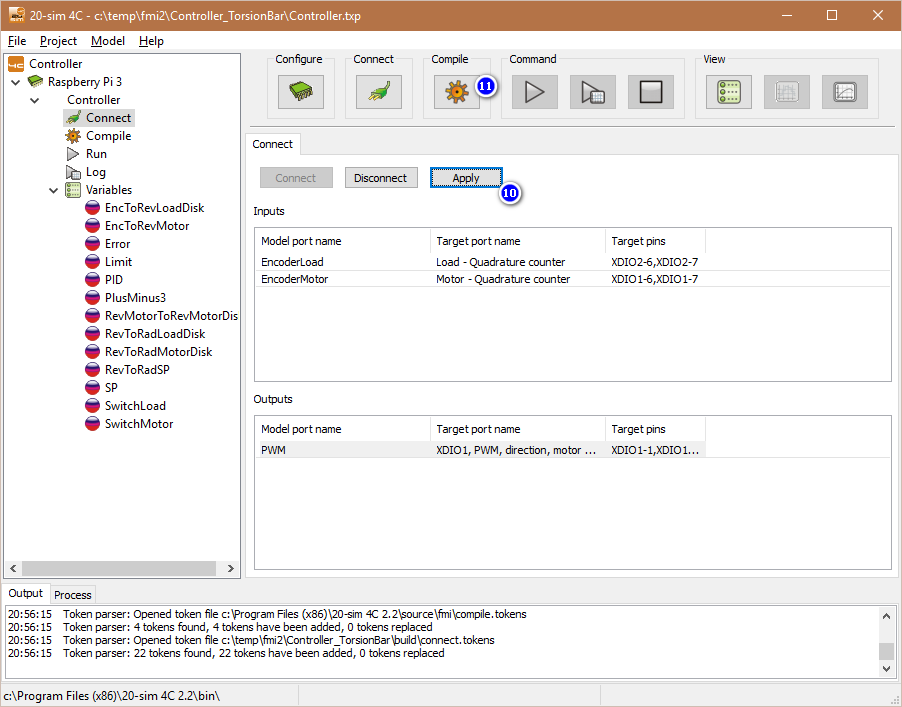
\includegraphics[width=\textwidth]{figures/20-sim-4C_connect_apply.png}}
	\caption{Apply the connections and compile the code.}
	\label{figure:20-sim-4C_connect_apply}
\end{figure}
%
\item Press the orange \textit{Compile} button (\autoref{figure:20-sim-4C_connect_apply}) to go to the \textit{Compile} phase.  This will compile the FMU source code and the additional 20-sim 4C source code into a real-time application.
%
\item When the compilation process is ready and successful, click the orange \textit{Command} button to configure the last task settings before uploading the compiled FMU to the Raspberry Pi (\autoref{figure:20-sim-4C_compile}.)
%
\begin{figure}[hpt]
	\centerline{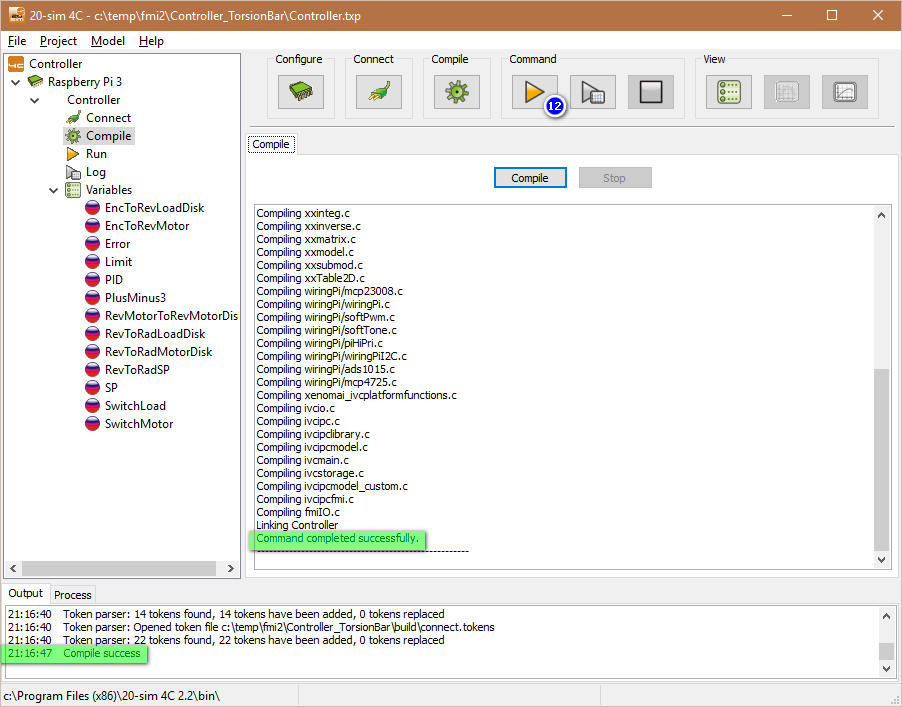
\includegraphics[width=\textwidth]{figures/20-sim-4C_compile.png}}
	\caption{Compilation phase.}
	\label{figure:20-sim-4C_compile}
\end{figure}
%
\item On the \textit{Configure Run} tab (\autoref{figure:20-sim-4C_run_settings}), you can specify the finish time of the FMU or disable it if it should run forever (until reboot/shutdown).  Ensure that the \textit{Discrete Time Interval} has a step size larger than 0.  This value is used as the time (step size) between two FMU ``doStep'' calls and determines the FMU calculation frequency.  The Raspberry Pi 3 is able to support step sizes as low as 0.00005 (20 kHz), but this depends on the FMU computation load and number of connected I/O pins.
%
\begin{figure}[hpt]
	\centerline{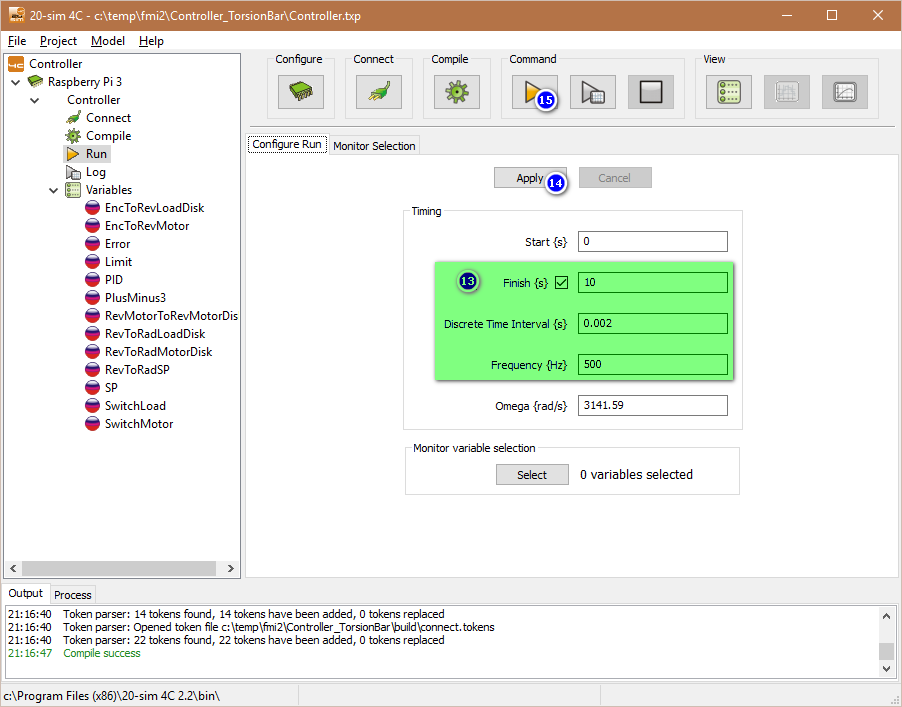
\includegraphics[width=\textwidth]{figures/20-sim-4C_run_settings.png}}
	\caption{Configure task run settings.}
	\label{figure:20-sim-4C_run_settings}
\end{figure}
%
\item Press the \textit{Apply} button to store the run settings.  The \textit{Command} button will turn green.
%
\item Click the \textit{Command} button to upload and start your FMU on the Raspberry Pi.  If everything is configured correctly, the FMU will start and 20-sim 4C will monitor its progress and the current value of the FMU variables.
%
\begin{figure}[hpt]
	\centerline{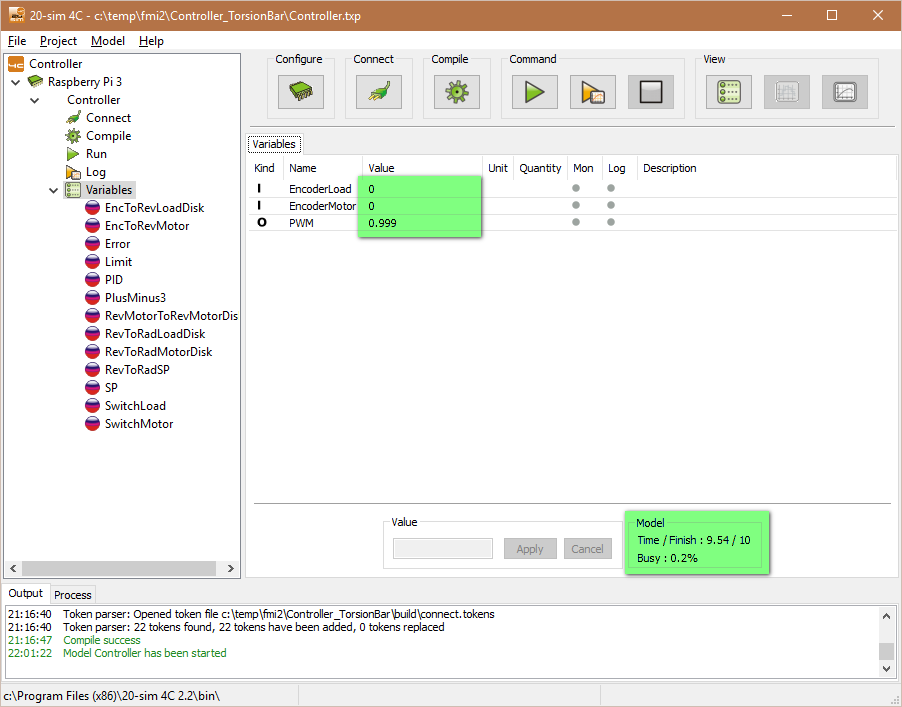
\includegraphics[width=\textwidth]{figures/20-sim-4C_running.png}}
	\caption{FMU is running.}
	\label{figure:20-sim-4C_running}
\end{figure}
%
\item It is also possible to show selected variables in a monitor plot.  You can enable monitoring of a signal by toggling the dot icon in the \textit{Mon} column to a monitor icon.
%
\item Click the large monitor icon on the button bar to show the monitor plot. An example of the monitor plot with three I/O signals is shown in \autoref{figure:20-sim-4C_monitoring_plot}.
%
\begin{figure}[hpt]
	\centerline{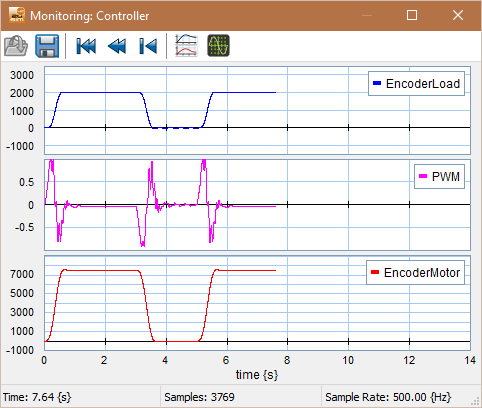
\includegraphics[width=0.7\textwidth]{figures/20-sim-4C_monitoring_plot.png}}
	\caption{Variable monitor.}
	\label{figure:20-sim-4C_monitoring_plot}
\end{figure}  
%  
\end{enumerate}
%
%
%
\subsubsection{Real-time toolwrapper FMU export}\label{sec:simulators:20sim4C:fmuexport}
For HiL simulation with a Raspberry Pi, 20-sim 4C is extended with FMU export functionality.
%
The 20-sim 4C FMU export option generates a real-time toolwrapper FMU for the currently loaded 20-sim 4C project.
%
This FMU can be used in the COE to interface the real-time FMU running on the Raspberry Pi with a standard COE co-simulation experment. 
%
Assuming a running application on the Raspberry Pi, FMU export can be performed as follows:
%
%
%
\begin{enumerate}
\item Co-simulation using a toolwrapper FMU uses the unconnected 20-sim 4C inputs.  Make sure that the desired co-simulation inputs are not connected during the 20-sim 4C \textit{Connect} phase (\autoref{figure:20-sim-4C_connect_apply}).
%
\item Export an FMU using the \textit{FMU Export} menu item.  Make sure that the ``Raspberry Pi 3'' target, or the 20-sim 4C  project (your FMU name,) is selected in the left tree.  This is required so that the FMU exporter can find the right 20-sim 4C project.
%
\item Select \textit{Export FMU} from the \textit{Project} menu item. See \autoref{figure:20-sim-4C_export_toolwrapper_fmu}.
% 
\begin{figure}[hpt]
	\centerline{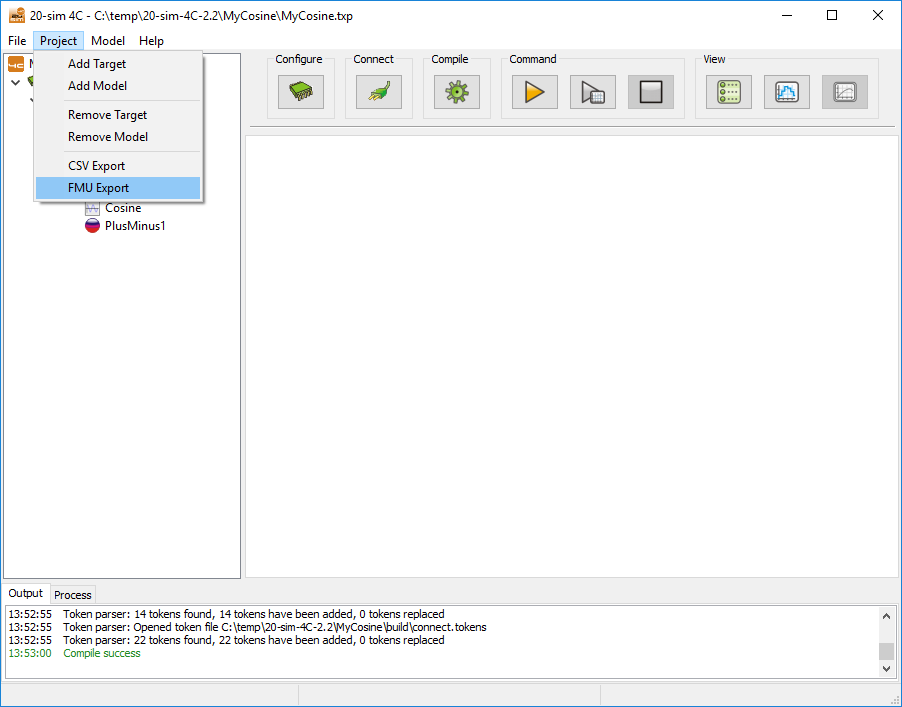
\includegraphics[width=\textwidth]{figures/20-sim-4C_export_toolwrapper_fmu.png}}
	\caption{Export toolwrapper FMU.}
	\label{figure:20-sim-4C_export_toolwrapper_fmu}
\end{figure}
%
\item A command-line window will be displayed showing status information of the FMU toolwrapper creation process.  See \autoref{figure:20-sim-4C_export_toolwrapper_fmu2}.
%
\begin{figure}[hpt]
	\centerline{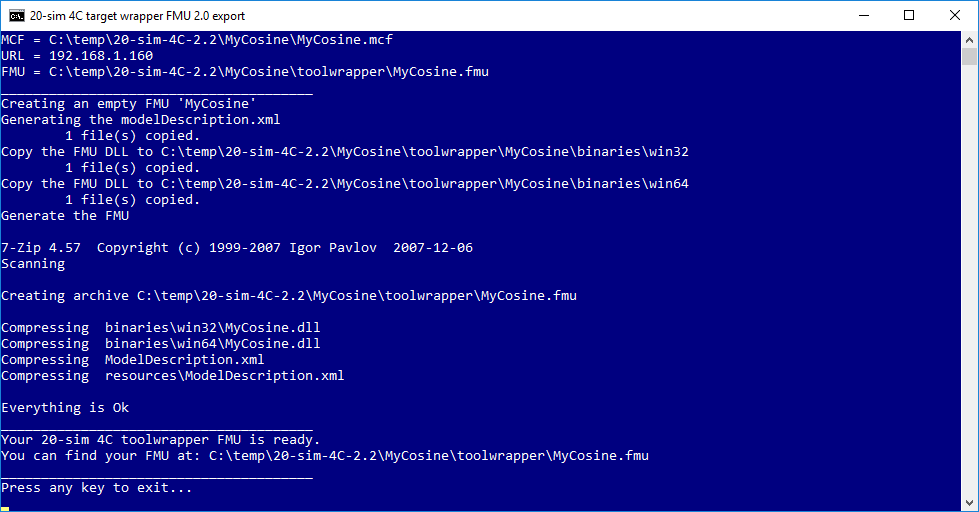
\includegraphics[width=\textwidth]{figures/20-sim-4C_export_toolwrapper_fmu2.png}}
	\caption{Toolwrapper FMU status.}
	\label{figure:20-sim-4C_export_toolwrapper_fmu2}
\end{figure}
%
\item This window can be closed after noting the location of the generated FMU.
%
\item The newly created FMU can be used in 32-bit and 64-bit Windows FMI co-simulators like the INTO-CPS COE.  Linux and MacOS X compatible versions are not yet available.
\end{enumerate}